% Carried over verbatim from monograph/main.tex (Study 1 record, 13 Sep 2026).
\chapter{SIPaKMeD classification rescore}\label{s1:ch:ch10_sipakmed_classification_rescore}

\section{Why re-run models rather than quote published scores?}

Published numbers are entangled with architectures, preprocessing, augmentations, and---most importantly---different splits. Quoting them would not isolate the quantity of interest. The rescore therefore trains six representative image classifiers under the same code path, preprocessing, optimizer family, epoch budget, seeds, and four fixed split protocols. The only intended change across protocols is the independence constraint and, for the explicitly size-matched control, the number of retained training crops.

The six families cover different inductive biases and capacities: ResNet-18 and ResNet-50~\cite{he2016resnet}, DenseNet-121~\cite{huang2017densenet}, MobileNet-V2~\cite{sandler2018mobilenetv2}, EfficientNet-B0~\cite{tan2019efficientnet}, and ViT-B/16~\cite{dosovitskiy2021vit}. Each ImageNet-pretrained head is replaced with a five-way linear classifier. Re-running all six also prevents the conclusion from depending on one especially favorable architecture.

\section{Inputs, augmentation, and optimization}

Every crop is decoded as RGB, converted to a tensor, and normalized by the ImageNet channel statistics. Training augmentation consists of a random resized crop to $224\times224$ with scale in $[0.8,1.0]$, a horizontal flip, and a vertical flip. Test preprocessing is a deterministic resize to $224\times224$. The code records the fully resolved split hash and configuration beside every result.

All classifiers use AdamW~\cite{loshchilov2019adamw}, cross-entropy loss, and a fixed learning rate. The retained endpoint is the final epoch; there is no separate validation split or post-hoc best-epoch selection. A run is valid only when the stored identifiers match its split, the final file is complete, and all reported quantities are finite. Table~\ref{s1:tab:classifier-hparams} gives the execution contract.

\begin{table}[H]
\centering
\caption{SIPaKMeD classifier execution settings.}
\label{s1:tab:classifier-hparams}
\begin{tabular}{ll}
\toprule
Item & Setting \\
\midrule
Architectures & ResNet-18/50, DenseNet-121, MobileNet-V2, EfficientNet-B0, ViT-B/16 \\
Initialization & ImageNet pretrained \\
Input & RGB, $224\times224$ \\
Loss & Five-class cross entropy \\
Optimizer & AdamW \\
Learning rate & $10^{-4}$, fixed \\
Weight decay & $10^{-4}$ \\
Batch size & 64 \\
Epochs & 20, final-epoch endpoint \\
Seeds & 17, 29, 43, 71, 101 \\
Primary metric & Test accuracy \\
Hardware & NVIDIA RTX A6000; at most three concurrent GPU jobs \\
\bottomrule
\end{tabular}
\end{table}

\section{Metric definitions}

For true class $y_i$ and prediction $\hat y_i$, accuracy is
\begin{equation}
\operatorname{Acc}=\frac{1}{N}\sum_{i=1}^{N}\mathbf{1}\{\hat y_i=y_i\}.
\end{equation}
For class $c$, with precision $P_c$ and recall $R_c$,
\begin{equation}
F_{1,c}=\frac{2P_cR_c}{P_c+R_c},\qquad
F_{1,\mathrm{macro}}=\frac{1}{C}\sum_{c=1}^{C}F_{1,c}.
\end{equation}
Balanced accuracy is the unweighted mean class recall,
\begin{equation}
\operatorname{BAcc}=\frac{1}{C}\sum_{c=1}^{C}\frac{TP_c}{TP_c+FN_c}.
\end{equation}
The preregistered primary endpoint is accuracy. Macro-F1 and balanced accuracy check that the direction is not a class-frequency artifact; they are not used to shop for a smaller $p$-value.

\section{Aggregate scores}

\begin{table}[H]
\centering
\caption{SIPaKMeD test accuracy (\%), mean $\pm$ sample SD over five seeds. \protocol{P1$'$} is numerically identical to \protocol{P1} because the frozen stratified crop split already contained the registered 3,239 training and 810 test observations.}
\label{s1:tab:classification-main}
\small
\begin{tabular}{lrrrr}
\toprule
Architecture & \protocol{P1} & \protocol{P1$'$} & \protocol{P2} & \protocol{P3} \\
\midrule
DenseNet-121 & 98.12$\pm$0.28 & 98.12$\pm$0.28 & 96.72$\pm$0.69 & 97.38$\pm$0.50 \\
EfficientNet-B0 & 97.78$\pm$0.49 & 97.78$\pm$0.49 & 96.69$\pm$1.49 & 97.41$\pm$0.71 \\
MobileNet-V2 & 97.41$\pm$0.45 & 97.41$\pm$0.45 & 95.16$\pm$1.50 & 96.20$\pm$0.93 \\
ResNet-18 & 97.19$\pm$0.59 & 97.19$\pm$0.59 & 96.00$\pm$0.89 & 96.35$\pm$1.28 \\
ResNet-50 & 97.51$\pm$0.47 & 97.51$\pm$0.47 & 96.79$\pm$0.42 & 96.27$\pm$0.53 \\
ViT-B/16 & 97.14$\pm$0.95 & 97.14$\pm$0.95 & 95.56$\pm$0.84 & 95.53$\pm$1.68 \\
\bottomrule
\end{tabular}
\end{table}

\begin{figure}[H]
\centering
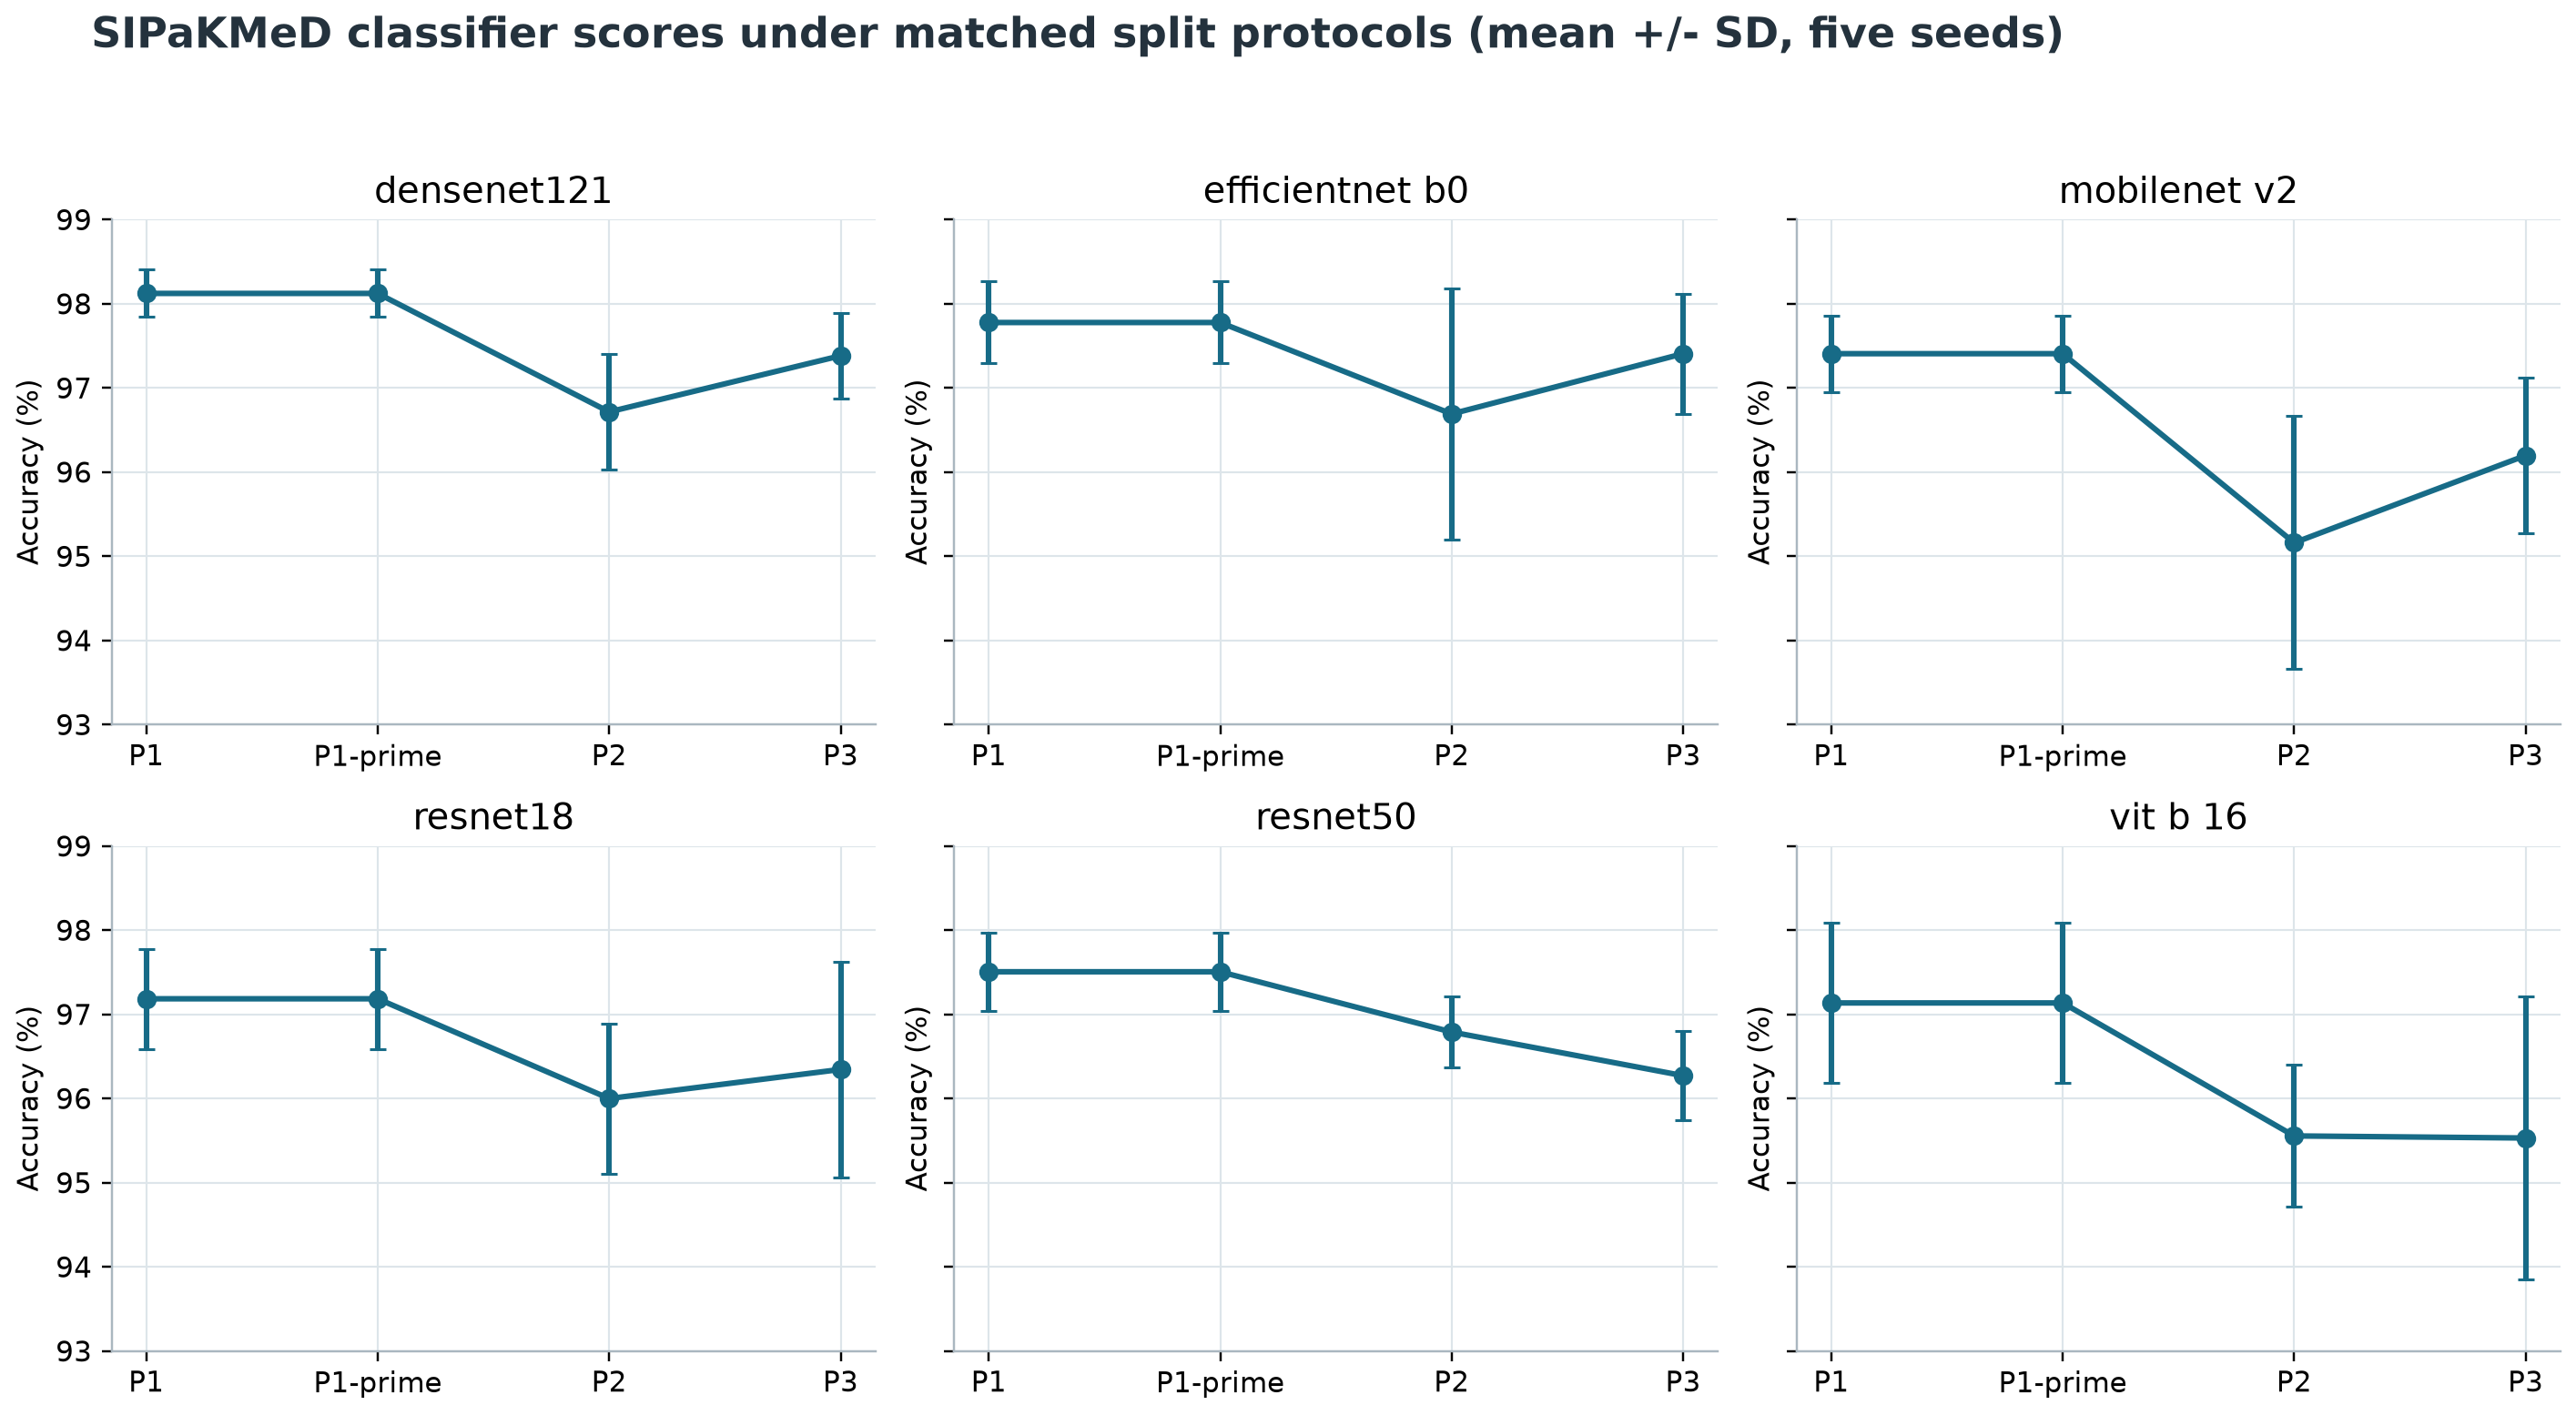
\includegraphics[width=\textwidth]{classification_protocol_scores.png}
\caption{All frozen SIPaKMeD accuracy observations. Lines connect the same architecture across protocols; points show individual seeds and bars show the mean.}
\label{s1:fig:classification-scores}
\end{figure}

The top score under \protocol{P1} is DenseNet-121 at 98.12$\pm$0.28\%. Under parent-disjoint \protocol{P2}, DenseNet-121 remains highest at 96.72$\pm$0.69\%, narrowly followed by ResNet-50. The key scientific observation is not which backbone wins; it is that all six paired \protocol{P1}$-$\protocol{P2} mean differences are positive.

\section{Matched contrasts, uncertainty, and the ordering failure}

For architecture $a$ and seed $s$, the primary paired difference is
\begin{equation}
d_{a,s}=100\left(\operatorname{Acc}_{a,s,\mathrm{P1}}-
\operatorname{Acc}_{a,s,\mathrm{P2}}\right)
\end{equation}
in percentage points. The paired standardized effect is Cohen's
\begin{equation}
d_z=\frac{\bar d}{s_d},
\end{equation}
where $s_d$ is the sample SD of the five seed-paired differences. Reported effect-size confidence intervals are seed-paired bootstrap intervals, so a bootstrap resample always keeps the two protocol results from a seed together. The test is a paired $t$-test because every registered five-difference vector passed its Shapiro--Wilk screen; the switch to Wilcoxon was reserved for a failed screen.

\begin{table}[H]
\centering
\caption{Primary SIPaKMeD \protocol{P1}$-$\protocol{P2} contrasts. The six paired $t$-tests form one preregistered BH family. CI is the paired-bootstrap 95\% interval for Cohen's $d_z$, not for the raw percentage-point mean.}
\label{s1:tab:classification-contrasts}
\small
\begin{tabular}{lrrrrr}
\toprule
Architecture & Mean$\pm$SD (pp) & 95\% CI for $d_z$ & $p$ & BH $q$ & $d_z$ \\
\midrule
DenseNet-121 & 1.41$\pm$0.90 & [0.985, 4.747] & 0.0251 & 0.1109 & 1.561 \\
EfficientNet-B0 & 1.09$\pm$1.85 & [$-$0.316, 4.668] & 0.2591 & 0.2591 & 0.588 \\
MobileNet-V2 & 2.25$\pm$1.63 & [0.809, 6.686] & 0.0370 & 0.1109 & 1.377 \\
ResNet-18 & 1.19$\pm$1.28 & [0.442, 2.365] & 0.1081 & 0.1511 & 0.922 \\
ResNet-50 & 0.72$\pm$0.83 & [0.085, 4.025] & 0.1260 & 0.1511 & 0.863 \\
ViT-B/16 & 1.58$\pm$1.70 & [0.057, 4.950] & 0.1059 & 0.1511 & 0.931 \\
\bottomrule
\end{tabular}
\end{table}

\begin{figure}[H]
\centering
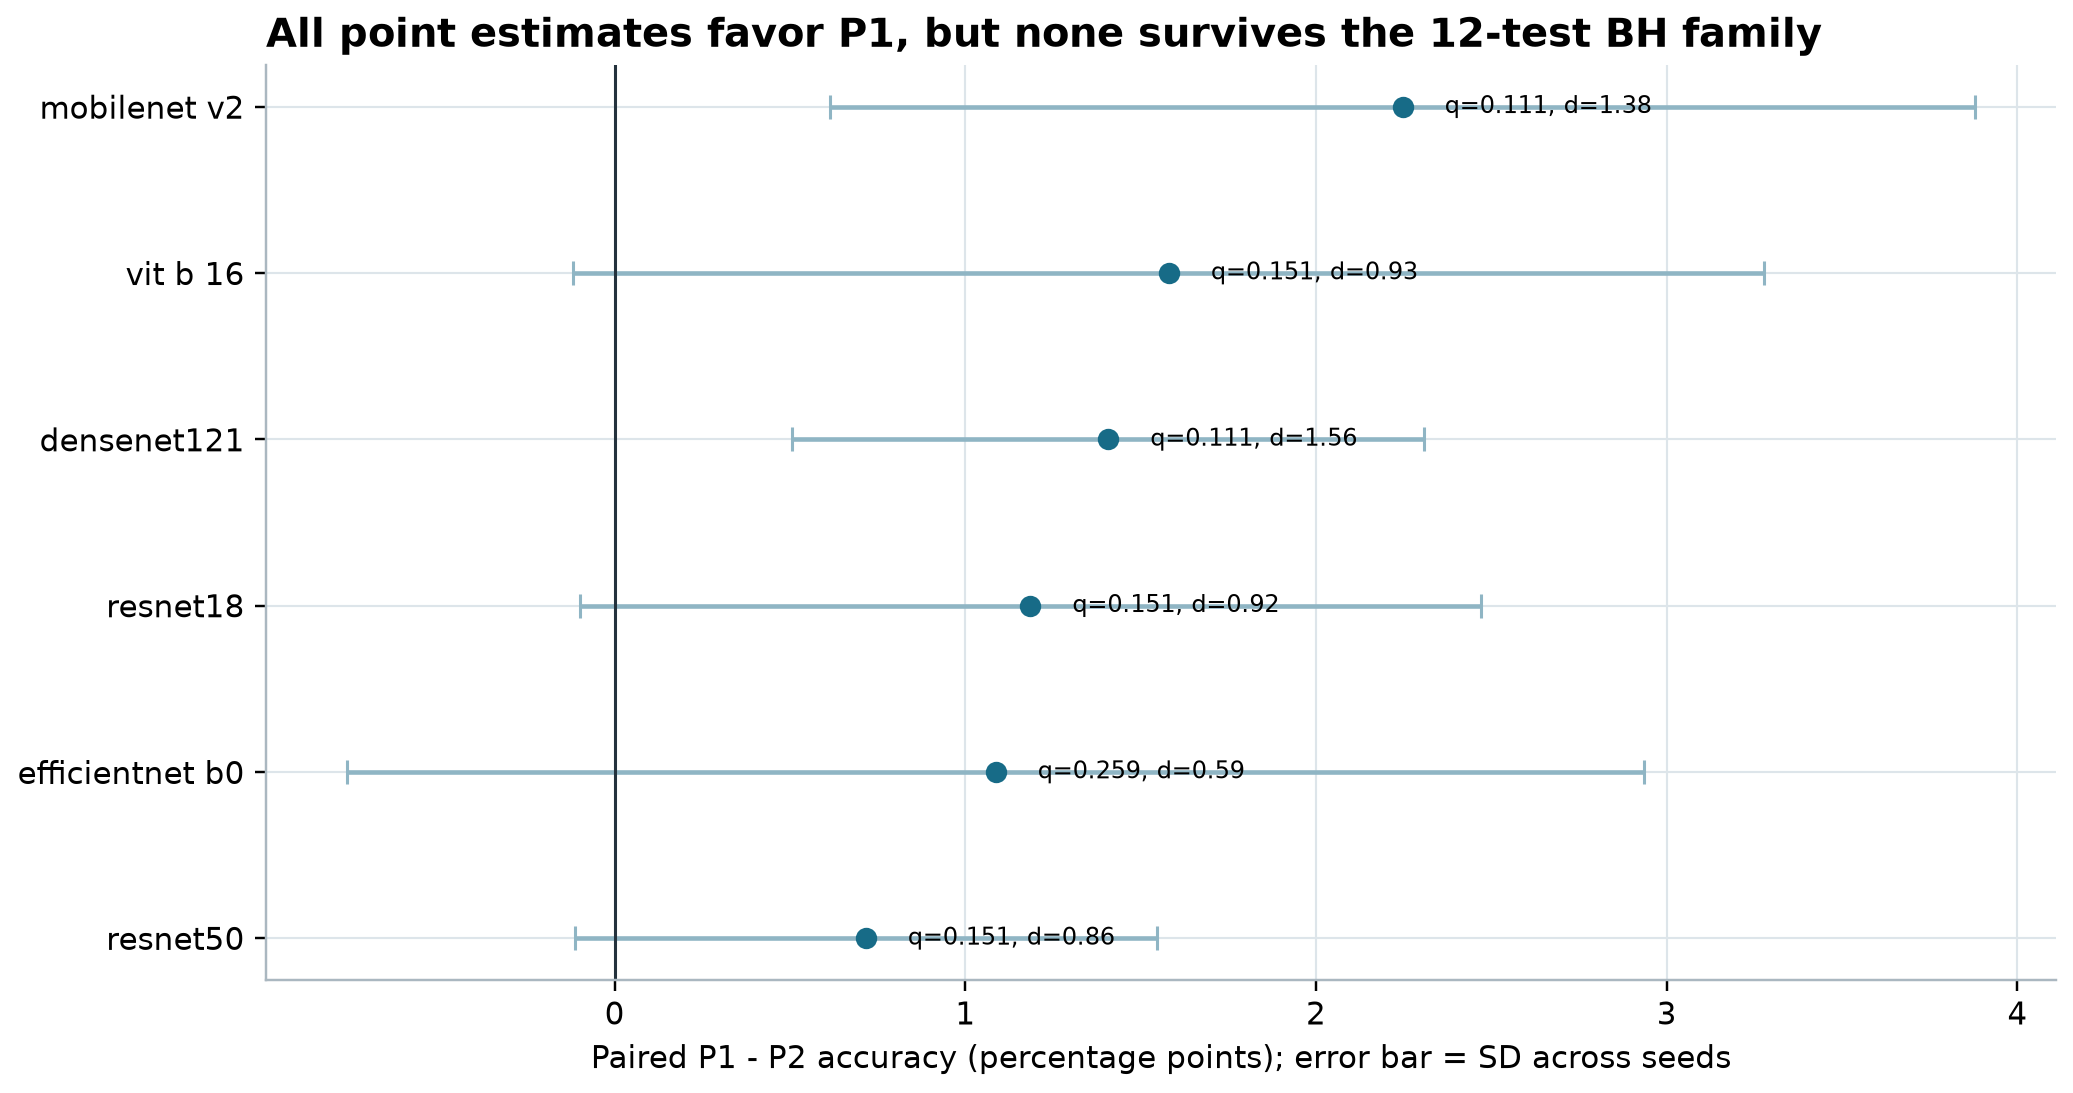
\includegraphics[width=\textwidth]{classification_delta_forest.png}
\caption{Paired \protocol{P1}$-$\protocol{P2} effects. Every mean favors the crop-level split, but none survives its preregistered multiplicity correction. The vertical line at zero marks no protocol effect.}
\label{s1:fig:classification-forest}
\end{figure}

\begin{figure}[H]
\centering
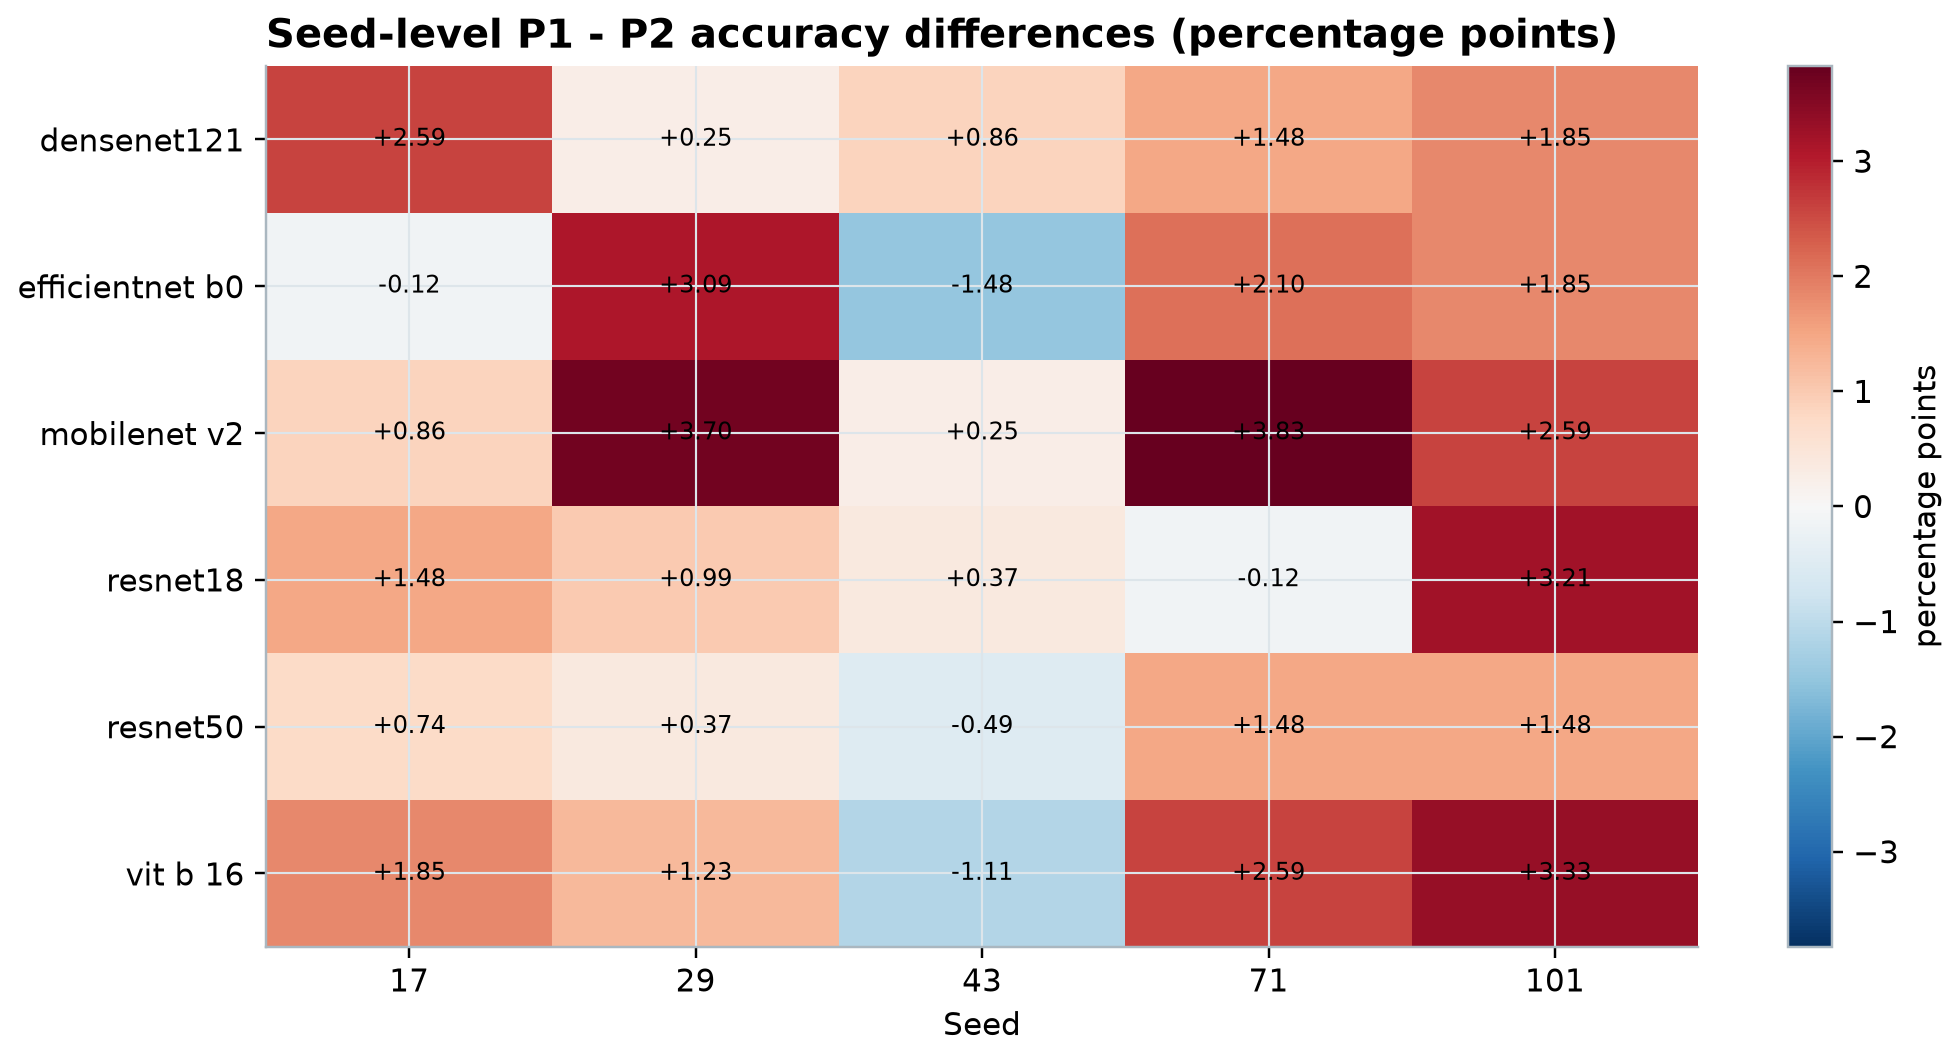
\includegraphics[width=\textwidth]{classification_seed_deltas.png}
\caption{Seed-level paired differences. This figure exposes the small effective sample size and the architecture-specific variability that an aggregate table can hide.}
\label{s1:fig:classification-seeds}
\end{figure}

The registered monotonicity expectation was \protocol{P3}$\leq$\protocol{P2}$\leq$\protocol{P1}. Only ResNet-50 and ViT-B/16 satisfy it. The other four improve from \protocol{P2} to \protocol{P3} by 0.35--1.04 points. Those reversals are not deleted or relabeled: the corresponding \protocol{P2}$-$\protocol{P3} differences are $-0.67$, $-0.72$, $-1.04$, $-0.35$, $+0.52$, and $+0.02$ points in table order, and none has an adjusted confirmatory claim.

\begin{figure}[H]
\centering
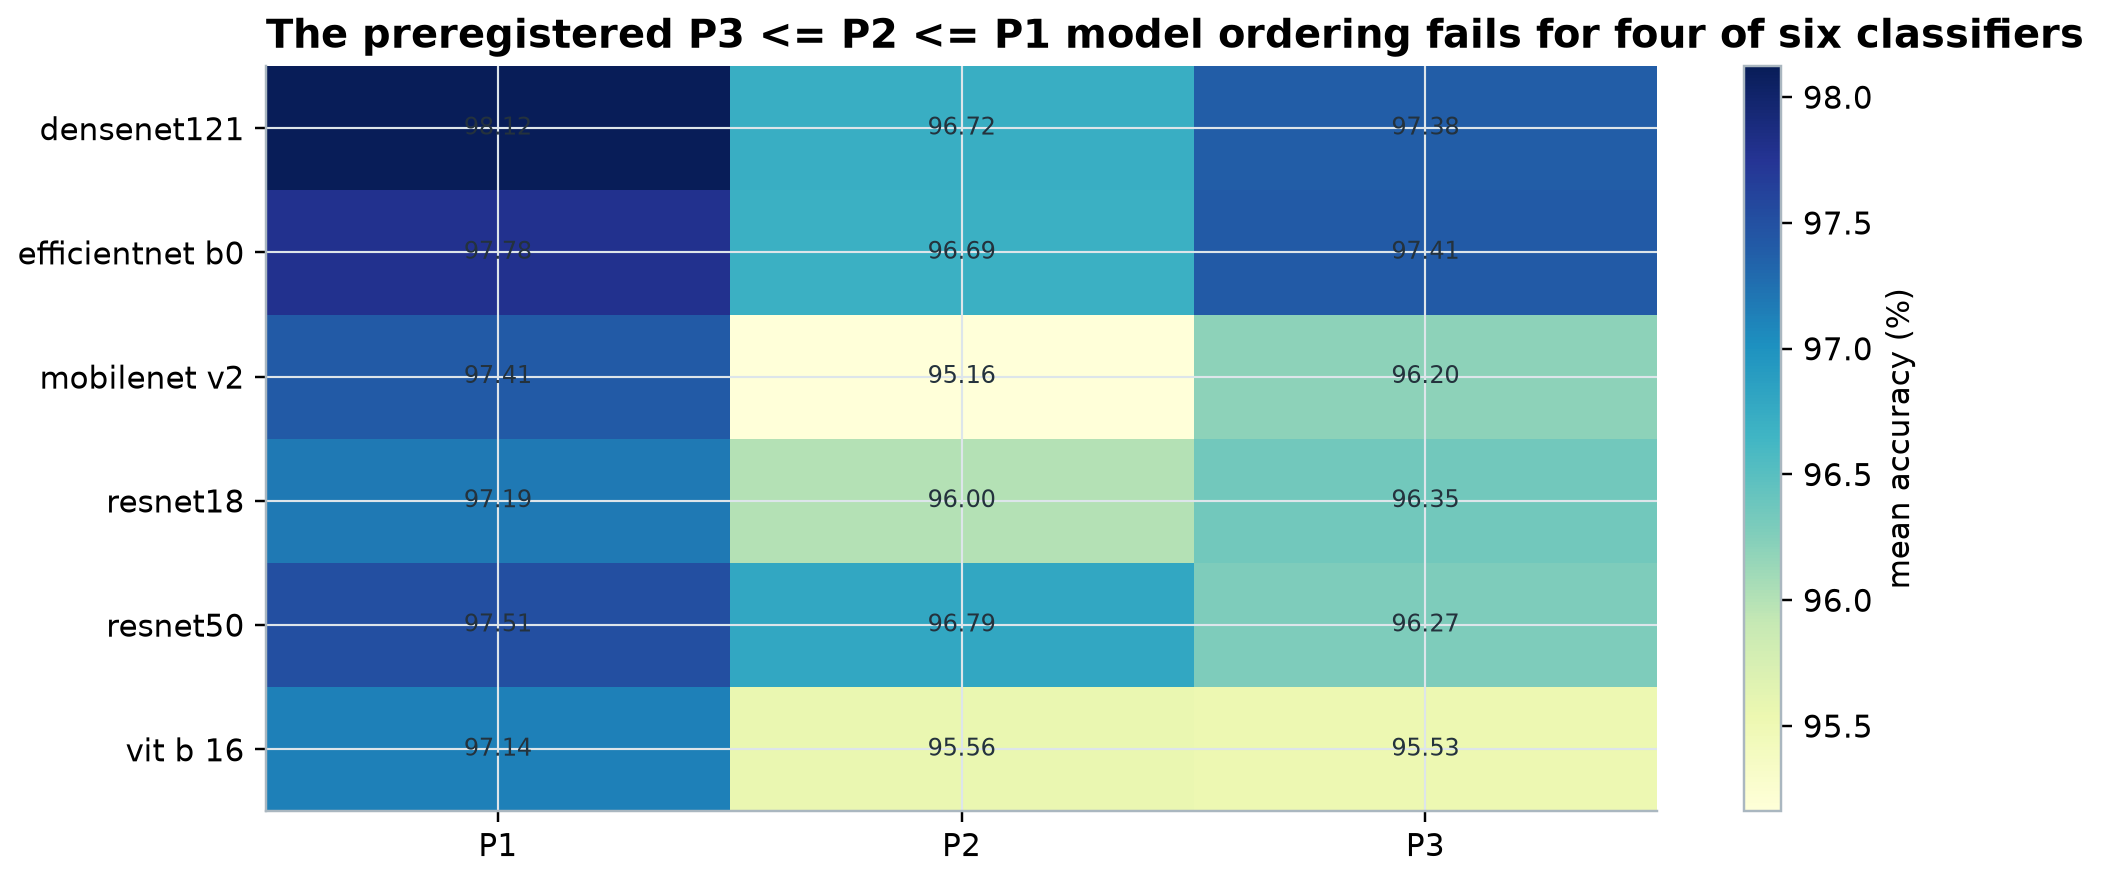
\includegraphics[width=\textwidth]{classification_ordering.png}
\caption{The registered ordering check. Cell values are the protocol means; the title records the gate outcome. Four of six architectures fail \protocol{P3}$\leq$\protocol{P2}$\leq$\protocol{P1}, so the acceptance contract correctly records one failed gate.}
\label{s1:fig:classification-ordering}
\end{figure}

Architecture ranks are also unstable across \protocol{P1} and \protocol{P2}: Kendall's $\tau=0.467$ with bootstrap interval [0.071, 0.733] and $p=0.2722$; four of the 15 architecture pairs reverse. This is a descriptive warning that a benchmark split can alter conclusions about model selection even when absolute score differences look modest.

\section{What the classification rescore does and does not show}

The same-sign result across six architectures is scientifically suggestive and consistent with the structural mechanism. The five-seed paired variability is nevertheless too large for any architecture to pass the six-test BH family. The correct report is therefore: \emph{crop-disjoint scores were higher on average for every tested classifier, by 0.72--2.25 percentage points, but the preregistered architecture-wise confirmatory family did not establish individual effects after multiplicity correction.}

No classifier confusion matrix appears because the frozen result schema retains aggregate test metrics and epoch histories, but not per-sample predictions or model checkpoints. Generating such a matrix now would require a new experiment after the declared research stop. Omitting it is more faithful than reconstructing or simulating unobserved cells.

\section{Training behavior and compute}

\begin{figure}[H]
\centering
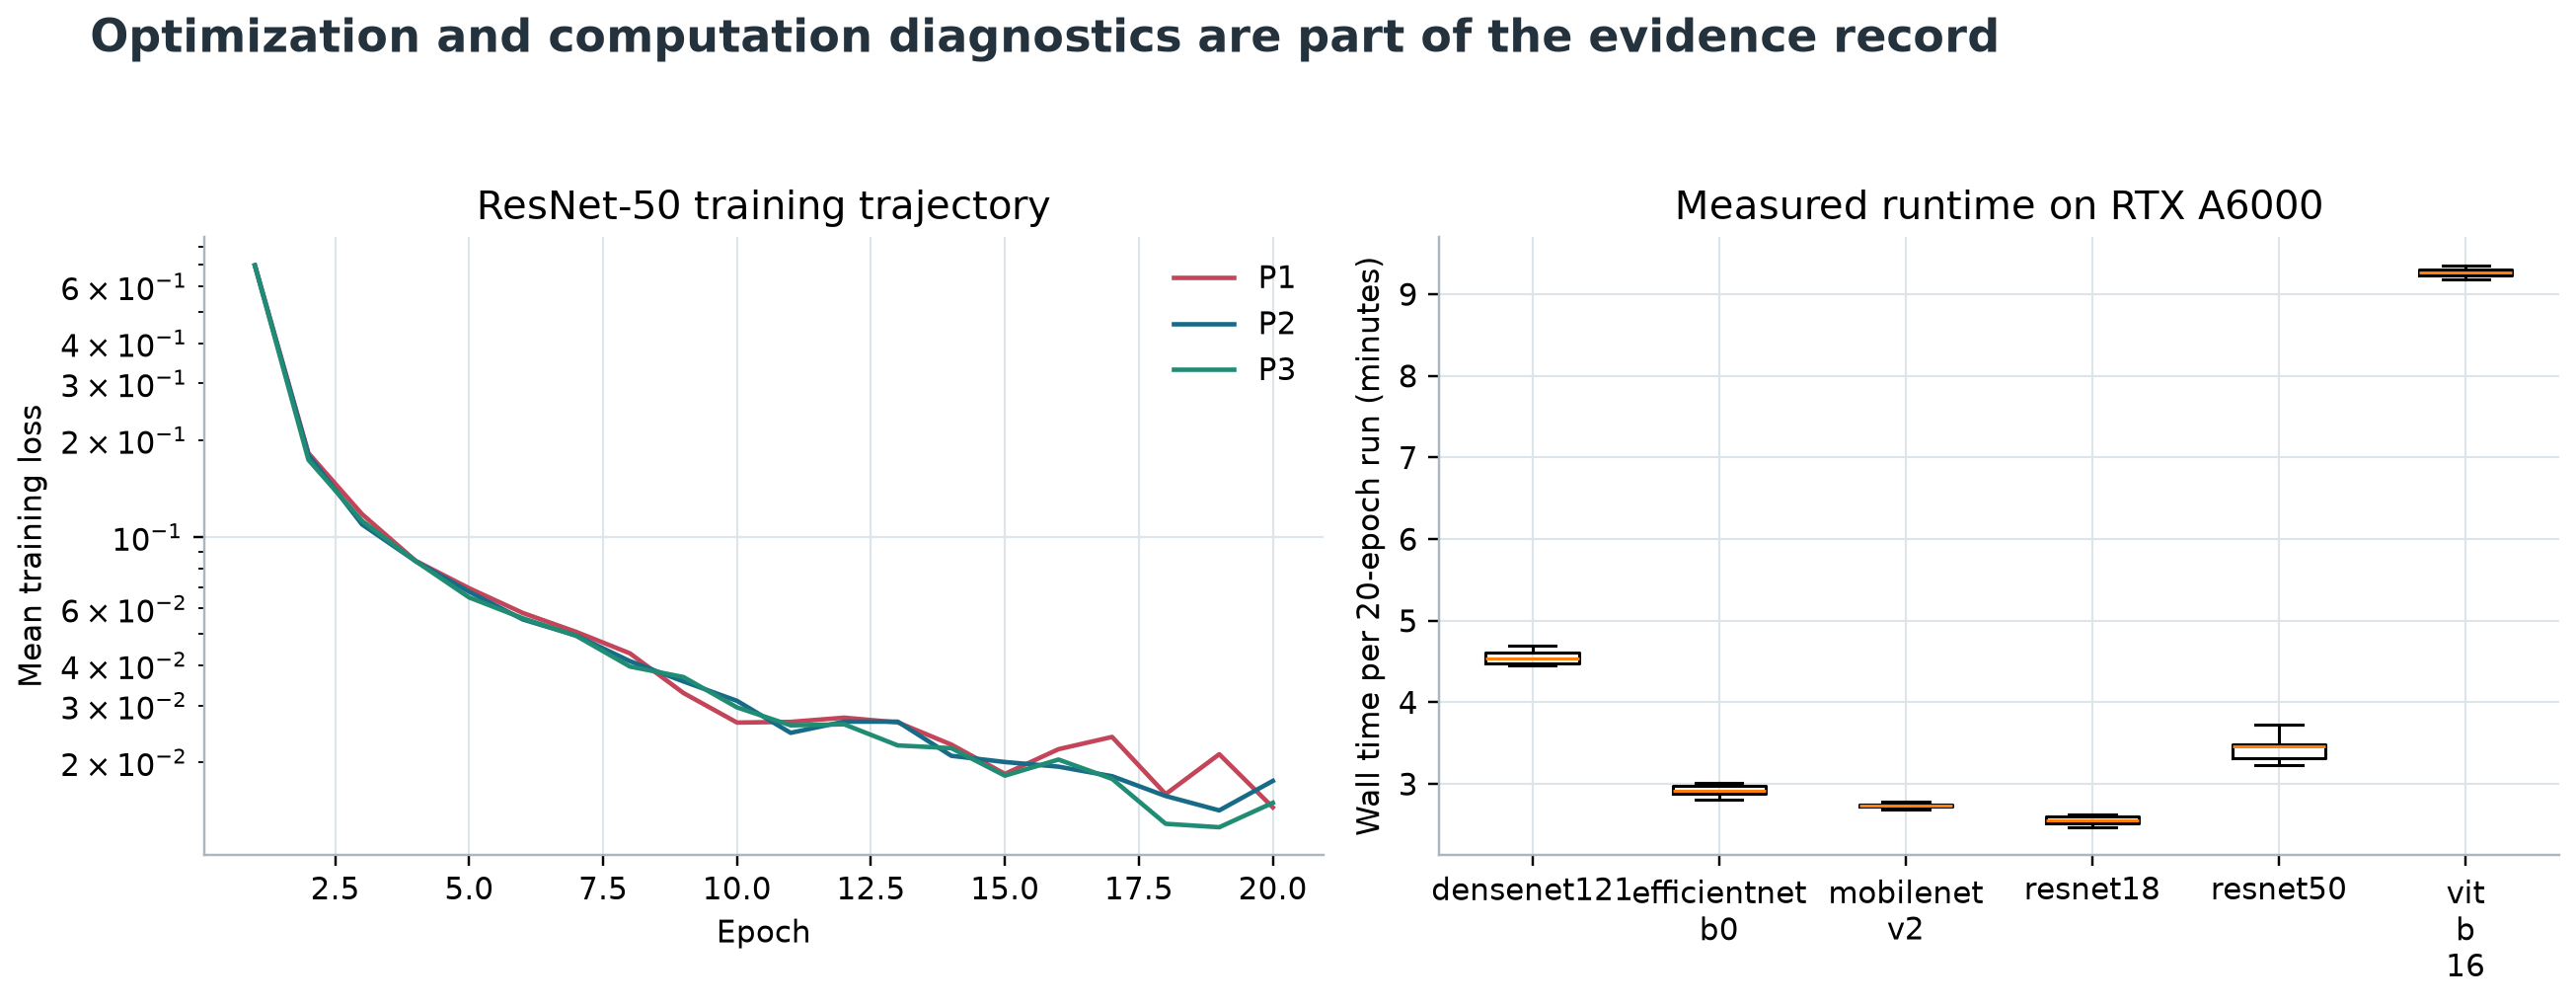
\includegraphics[width=\textwidth]{classification_training_runtime.png}
\caption{Classifier wall-clock summaries from the retained run JSON files. These are same-system measurements and should not be compared to timings reported on unrelated hardware.}
\label{s1:fig:classification-runtime}
\end{figure}

The 120 retained classification runs consumed 8.48 summed run-hours. Because up to three jobs ran concurrently, this is computational work, not elapsed calendar duration. Shorter wall time does not imply a more accurate or better-calibrated model; it is included so the execution cost is auditable.
